\documentclass[final,11pt,times,twocolumn]{elsarticle}
\usepackage[top = 4cm, bottom = 3cm, right = 2cm, left = 2cm, a4paper]{geometry}
\usepackage{amssymb}

\begin{document}
\begin{frontmatter}
\title{Uranium diboride, the potential candidates of ATF, feature and application \\ \LaTeX}
\begin{abstract}
It is universally acknowledged that power generation is most fundamental facility required by every industry, as almost all things require electricity to work. Among all the methods of electricity generation, nuclear power always faces considerable scrutiny. Undoubtedly, nuclear power brings about feelings of fear and unknown horror, especially after the accidents at Fukushima and Chernobyl. Such concerns are not unreasonable, as people's fear of nuclear power is a good measure to prevent accidents from happening. However, Taiwan people are too afraid of using this technology, turns out the result is miss out the opportunity to improve our ecosystem and make it more environmentally friendly. In this research, I would put the focus on the potentially fuel, Uranium diboride (UB$_{2}$), an interesting fuel that nowadays are research to be an ATF candidate fuel. Its physical properties also make it suitable for use in GEN-IV reactors, which require high standards to reaction. All of these factors make UB$_{2}$ show on my eyes, and this research aims to explore its potential.
\end{abstract}

\begin{keyword}
ATF, Uranium diboride, GEN-IV reactors
\end{keyword}

\end{frontmatter}

\section{Introduction}
Uranium diboride is potentially material which
on closely debating to be the next generation re-
actors fuel, expecialy known as ATF. UB2 have
unique talent to play a important role in these fu-
ture plan. ATF purpose almost seems like make
increasing the reactors power up-rates, longer cy-
cle lengths, improved performance due to lowered
thermal gradients across the fuel pellet reduced
stored energy in the core, and allow for increased
coping time during accident scenarios.

\begin{figure}[ht]
    \centering
    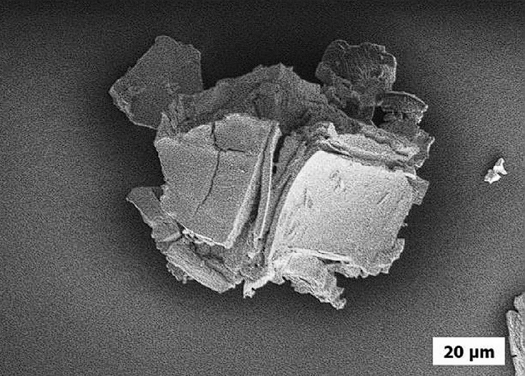
\includegraphics[width = 5.75cm]{UB2 Micrographs.png}
    \caption{UB2 Micrographs Picture}
\end{figure}

\section{The nuclear}
Because this paper more like a class report than a real paper and not very rigorous, so before
introduce and futher more research UB$_{2}$, I liked to totally
explain how the nuclear make our life so dramatic.

\subsection{History}
Recently, the Movie "Oppenheimer" was release(24.07.2023)

\section{Physical properties}
In many candidate of ATFs material, the Uranium 
diboride has higher Uranium density than
the others. Also, it has better thermal conduc-
tivity that make itself have lower fuel centre-line
temperatures on working, result in many positive
effect such like: reduce the rate of temperature-
dependent release of fission products, reduce the
energy stored inside the fuel (This properties also
is the most important that the UB2 need.)

\end{document}
\endinput

